\documentclass[../main.tex]{subfiles}
\graphicspath{{img},{img/ink},{ink}}

\begin{document}

\begin{tcolorbox}[
    width=\textwidth,
    height=\textheight,
    title=Versuch: Newtonsche Bewegungsgleichung,
    fonttitle=\Large,
    before title=\vspace{0.2cm}, after title=\vspace{0.2cm},
    colback=white,
    title filled=true, 
    colbacktitle=mygray,
    colframe=black,
    coltitle=black,
    ]

    \vspace{0.2cm}
    \textbf{Klassenstufe}: 9/10

    \vspace{0.3cm}

    \textbf{Fachlicher Bezug}: Experimentelle Bestätigung des Newtonschen Axioms $F=m\cdot a$

    \vspace{0.3cm}

    \textbf{Material}: 
    Sensor-CASSY, 
    BMW-Box + Bewegungsaufnehmer,
    Laptop mit CASSY-Lab, 
    Haltemagnet, 
    Stativmaterial, 
    Experimentierkabel,
    Luftkissenfahrbahn,  
    Luftversorgung,
    mehrere identische Massestücke (z.B. 10g),
    Faden, 
    Wagen (250g und 500g)

    \begin{center}
        \includegraphics[width=1\textwidth]{img/versuchsaufbau}
    \end{center}

    \textbf{Aufbau}: Der Haltemagnet lässt sich direkt über das Sensor-CASSY mit Strom versorgen. Durch ein Potentiometer zwischen den Anschlüssen kann die Versorgungsspannung so eingestellt werden, dass der Wagen gerade noch festgehalten wird. Der Bewegungsaufnehmer wird über die obere Buchse der BMW-Box am Sensor-CASSY angeschlossen. 

    \vspace{0.3cm} 
    \textbf{Durchführung}: Die qualitative Bestätigung des Bewegungsgesetztes erfodert den Nachweis der Proportionalitäten:
    \begin{enumerate}
        \item $F \sim a$ $(m=\text{const})$: \textbf{Die beschleunigte Masse besteht immer aus der Gesamtheit des Wagens und allen verwendeten Massestücken}. Im ersten Durchgang beschleunigt die Gewichtskraft von einem Massestück. Mit jedem weiteren Durchgang wird die Gewichtskraft durch Hinzufügen von Massestücken linear erhöht. 
        \item $a \sim \frac{1}{m}$ $(F=\text{const})$: In jedem Durchgang beschleunigt die Gewichtskraft von einem Massestück. Im ersten Durchgang wird eine Masse von 260g (Waagen 250g + Massestück 10g) beschleunigt. Im nächsten Durchgang muss dann eine Masse von 520g (Waagen 500g + 2 Massestücke 10g) beschleunigt werden.  
    \end{enumerate}

    \vspace{0.3cm}
    \textbf{Ergebnis}: Die Bestimmung der Beschleungigung erfolgt in CASSY-Lab über ein Steigungsdreieck im $v(t)$-Diagramm oder über Mittelwertbildung im $a(t)$-Diagramm. Durch geeignete Wahl der Proportionalitätskonstanten folgt die Newtonsche Bewegungsgleichung. 

    \vspace{0.3cm}
    \textbf{Didaktische Bemerkungen}: In der Software Cassy-Lab ist bereits ein entsprechendes Beispiel \glqq Bewegungen auf der Luftkissenfahrbahn (Newtonsche Bewegungsgleichung)\grqq{} hinterlegt. Dabei werden die Kurven der einzelnen Durchgänge gemeinsam in einem Koordinatensystem dargestellt.     

\end{tcolorbox}


\end{document}
